In this section, we describe the KEM-based variant of the Signal protocol that is the subject of our symbolic analysis. As explained in the introduction, the Signal protocol is separated in two sub-protocols providing different functionalities, we respect this separation for this KEM-based variant in order to facilitate its analysis and clearly identify the contribution of each sub-protocol in the security of the whole protocol. The first sub-protocol named PQ-X3DH is used as authenticated key agreement while the second one named KEM-double-ratchet is used for secure instant messaging by refreshing the session key at each time a message is sent.

\subsection{The PQ-X3DH Protocol}

\begin{figure}[ht!]
\centering
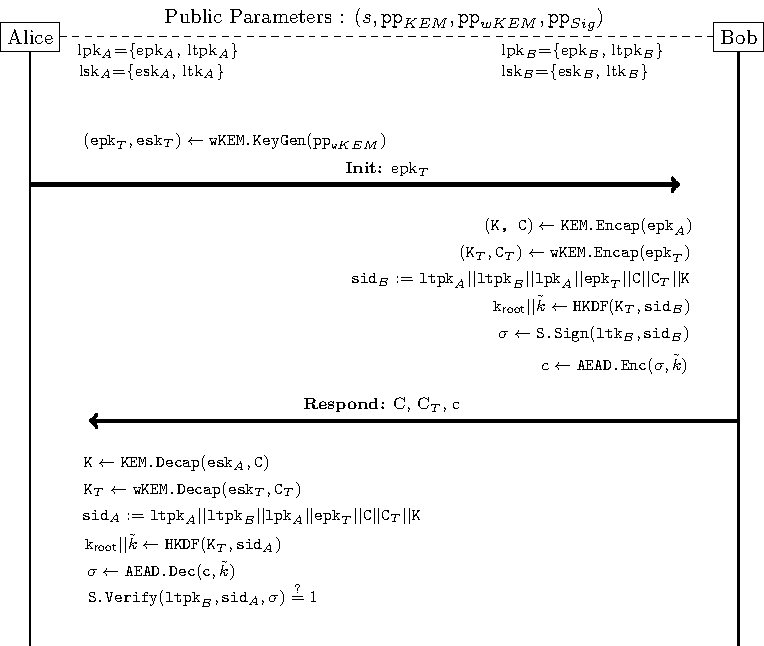
\includegraphics[width=\textwidth]{KEM_X3DH_only_sign}    
\caption{The PQ-X3DH protocol.}
\label{X3DH}
\end{figure}

X3DH~\cite{X3DH} is an asynchronous protocol that generates a shared secret between the communicating parties to initialize their communication as well as authenticate themselves. It fully authenticates the receiver Bob and partially authenticates the initiator Alice. It is called asynchronous because both parties can initiate the connection while the other is offline. Such property provides flexibility but could completely break the protocol in the case of a malicious server. Apart from such a case the asynchronous protocol is highly secure. We consider here the PQ-X3DH presented in~\cite{DBLP:conf/pkc/HashimotoKKP21} which preserve the security properties of the classical protocol and we focus on the variant of PQ-X3DH that does not use a signature to fully authenticate Alice. The motivation for this change is to allow Alice to deny having taken part in the exchange, in the same way that Bob can deny it thanks to the encryption of his signature.
%%%%%%%%%%%%%%%%%%%%%%%%%%%%%%%%%%%%%%%%%%%%%%%%%%%%%%%%%%%%%%%%%%%%%%%%%%%%%%%%%%%%%%%%%%%%%%%%%%%%

%%%%%%%%%%%%%%%%%%%%%%%%%%%%%%%%%%%%%%%%%%%%%%%%%%%%%%%%%%%%%%%%%%%%%%%%%%%%%%%%%%%%%%%%%%%%%%%%%%%%
The PQ-X3DH sub-protocol is presented in Figure~\ref{X3DH}. Two key 
encapsulation mechanisms, $\KEM$ and $\wKEM$, are employed as building blocks 
in this key agreement protocol. $\wKEM$, which is $\indcpa$ secure, is for 
ephemeral use. $\KEM$ is $\indcca$ secure here. Tamarin considers the 
public-key encryption as ideal (thus $\indcca$), but for an ephemeral use, 
$\indcpa$ is sufficient.

%\par
%
%vecos With the $\KeyGen$ algorithm of the $\wKEM$ primitive, Alice generates an encapsulation key $\epkT$ and a decapsulation key $\eskT$, the encapsulation key being sent to Bob.\par

%vecos With that key, and with the long-term encapsulation key $\eskA$ of Alice, Bob creates two pairs $(\K, \C)$ and $(\KT, \CT)$, each containing a session key and the associated ciphertext. Bob then constructs the session identifier $\sidB$ by concatenating a few keys and ciphertexts belonging to the current session. That identifier is then used by Bob, alongside the session key $\KT$, as input of a key derivation function  based on a $\HMAC$ primitive ($\HKDF$) to derive a concatenation of the two following keys: $\kroot$, the initial common key used in the double ratchet algorithm, and $\ktilde$, used in the next steps with the authenticated encryption primitive. $\sidB$ is also signed by Bob which guarantees the uniqueness of this session after verification, and this signature $\macrosigma$ is encrypted with an authenticated encryption scheme ($\AEAD$) and send to Alice, with the two other ciphertexts previously produced by Bob using the key encapsulation mechanisms $\KEM$ and $\wKEM$.\par

%vecos After recovering $\K$ and $\KT$ using $\KEMDecap$ and $\wKEMDecap$ with its decapsulation keys $\eskA$ and $\eskT$, Alice generates, as Bob did, a session identifier $\sidA$ and the concatenation of the keys $\kroot$ and $\ktilde$. Then, with this latter key, she decrypts $\macroc$ to recover the signature $\macrosigma$ whose correspondence with $\sidA$ is verified with the signing key $\ltpkB$ of Bob.\par
%%%%%%%%%%%%%%%%%%%%%%%%%%%%%%%%%%%%%%%%%%%%%%%%%%%%%%%%%%%%%%%%%%%%%%%%%%%%%%%%%%%%%%%%%%%%%%%%%%%%


%%%%%%%%%%%%%%%%%%%%%%%%%%%%%%%%%%%%%%%%%%%%%%%%%%%%%%%%%%%%%%%%%%%%%%%%%%%%%%%%%%%%%%%%%%%%%%%%%%%%
%The KEM-X3DH sub-protocol is presented in Fig.~\ref{X3DH} and uses the following functions and
%objects:
%\begin{itemize}
%    \item KEM functions (KeyGen, Encap, Decap) and wKEM for ephemeral KEM.
%    \item AEAD: an authenticated encryption scheme with associated data (Enc, Dec).
%    \item signature functions (Sign, Verify).
%    \item HKDF: a keyed key derivation function.
%    \item sid: session id (it is used as a transcript between the users).
%\end{itemize}
%%%%%%%%%%%%%%%%%%%%%%%%%%%%%%%%%%%%%%%%%%%%%%%%%%%%%%%%%%%%%%%%%%%%%%%%%%%%%%%%%%%%%%%%%%%%%%%%%%%%

\begin{figure}[htbp]
    \centering
    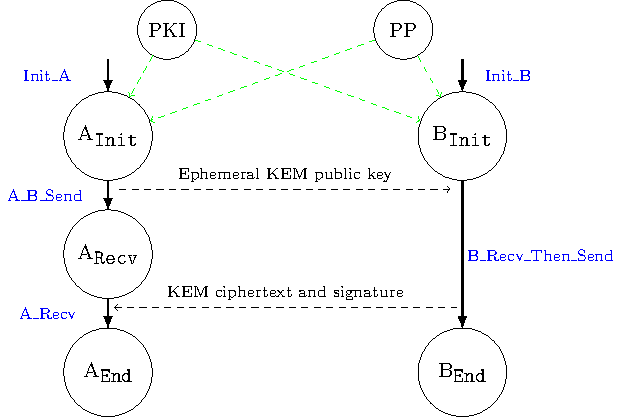
\includegraphics[scale=0.85]{Graph_X3DH.pdf}
    \caption{Graph of the Tamarin PQ-X3DH model.}
    \label{fig:GraphX3DH}
\end{figure}
%%%%%%%%%%%%%%%%%%%%%%%%%%%%%%%%%%%%%%%%%%%%%%%%%%%%%%%%%%%%%%%%%%%%%%%%%%%%%%%%%%%%%%%%%%%%%%%%%%%%

%%%%%%%%%%%%%%%%%%%%%%%%%%%%%%%%%%%%%%%%%%%%%%%%%%%%%%%%%%%%%%%%%%%%%%%%%%%%%%%%%%%%%%%%%%%%%%%%%%%%
%\subsubsection{Tamarin model.} We model the KEM-X3DH protocol in Tamarin with three core rules. Each user first gather mandatory information provided by the Public Key Infrastructure (PKI) and the global public parameters in their initialization. It is done by the two rules \texttt{Init\_A} and \texttt{Init\_B} presented in Fig.~\ref{fig:GraphX3DH}. Then the initiator sends an ephemeral public key to initiate a KEM with \texttt{A\_B\_Send}. When the responder receives the message, he encapsulates two key to form two pairs of secret and challenge. With these secrets, the responder derives a session key that will be used by both parties to communicate afterward. Furthermore he builds a signature that will be sent to the Initiator to authenticate himself. The last message is composed of the challenges made from the encapsulation and from the encoding of the signature.

%To supplement it, there are four subsequent rules whose two are modelling the Public Key Infrastructure (PKI) and the Public Parameters (PP) and two are modelling the adversary capacities. PKI models the public key infrastructure, it assigns only once a long term key with an ephemeral key to an user. Instead of handling non-replayability with a batch of ephemeral one-time keys we directly use restrictions so that the keys can only be used once.
%Since we are adapting the model in~\cite{DBLP:conf/pkc/HashimotoKKP21} to Tamarin, none of the public parameters are particularly useful as they are mostly used as seed but they allow for an understanding of the link between our Tamarin model with the one depicted in~\cite{DBLP:conf/pkc/HashimotoKKP21}. The two last rules model the advantage of the adversary. The protocol uses two secret information: the secret long term key and the secret ephemeral key where each of these keys can be revealed by the adversary.
%%%%%%%%%%%%%%%%%%%%%%%%%%%%%%%%%%%%%%%%%%%%%%%%%%%%%%%%%%%%%%%%%%%%%%%%%%%%%%%%%%%%%%%%%%%%%%%%%%%%

%%%%%%%%%%%%%%%%%%%%%%%%%%%%%%%%%%%%%%%%%%%%%%%%%%%%%%%%%%%%%%%%%%%%%%%%%%%%%%%%%%%%%%%%%%%%%%%%%%%%
\subsubsection{Tamarin model.} Since Tamarin has no built-in KEM we replace the KEM with an asymmetric encryption scheme encrypting a fresh ephemeral key. The two approaches are equivalent considering the idealization of cryptographic primitives used in Tamarin. Our model for the PQ-X3DH protocol is represented as the state machine in Figure~\ref{fig:GraphX3DH} with nine transition rules:
\begin{compactitem}
\item \texttt{PKI} and \texttt{PP}: these rules formalize the Public Key Infrastructure (PKI), the Public Parameters (PP). PKI assigns only once a long term key with an ephemeral key to a user. Instead of handling non-replayability with a batch of ephemeral one-time keys we directly use restrictions to ensure the a key can only be used once.
\item \texttt{Init\_A} and \texttt{Init\_B}: each user get from PKI and PP the public parameters and public keys needed for the PQ-X3DH protocol.
\item \texttt{A\_B\_Send}: Alice sends an ephemeral public key to initiate a key encapsulation.
\item \texttt{B\_Recv\_Then\_Send}: Bob receives Alice's ephemeral public key, encapsulates two secret keys into two KEM ciphertexts, one with Alice's ephemeral public key and wKEM, the other by using Alice's long-term public key and KEM. Bob also sign the protocol transcript and send his signature encrypted with an AEAD scheme.
\item \texttt{A\_Recv}: Alice receives Bob's ciphertext and signature and derives a session key that will be used by Alice and Bob to communicate. Then, she decrypts and verifies the signature.
\item \texttt{RevealE}: Reveals to the attacker the ephemeral secret keys.
\item \texttt{RevealL}: Reveals to the attacker the long-term secret keys.
\end{compactitem}
%%%%%%%%%%%%%%%%%%%%%%%%%%%%%%%%%%%%%%%%%%%%%%%%%%%%%%%%%%%%%%%%%%%%%%%%%%%%%%%%%%%%%%%%%%%%%%%%%%%%

\subsection{The KEM-double-ratchet Protocol}

%%%%%%%%%%%%%%%%%%%%%%%%%%%%%%%%%%%%%%%%%%%%%%%%%%%%%%%%%%%%%%%%%%%%%%%%%%%%%%%%%%%%%%%%%%%%%%%%%%%%
 %The Double-Ratchet protocol allows two parties to continuously exchange securely with fresh keys while saving the authentication made by the KEM-X3DH initialization. It is formalized with two categories of exchanges:
%\begin{description}
%    \item[Asymmetric] An \emph{asymmetric} exchange is an exchange in the most primary meaning. If we have two parties $A$ and $B$, then we obtain the pattern: Send\_A $\rightarrow$ Recv\_B $\rightarrow$ Send\_B $\rightarrow$ Recv\_A $\rightarrow$ Send\_A $\rightarrow$ \dots
%    \item[Symmetric] A \emph{symmetric} exchange is a set of messages from one sender, we obtain the pattern: Send\_A $\rightarrow$ Send\_A $\rightarrow$ Send\_A $\rightarrow$ \dots
%\end{description}

%Most protocols using the double ratchet consider asymmetric exchanges, hence we focus in this paper on asymmetric exchanges too.
%%%%%%%%%%%%%%%%%%%%%%%%%%%%%%%%%%%%%%%%%%%%%%%%%%%%%%%%%%%%%%%%%%%%%%%%%%%%%%%%%%%%%%%%%%%%%%%%%%%%

%%%%%%%%%%%%%%%%%%%%%%%%%%%%%%%%%%%%%%%%%%%%%%%%%%%%%%%%%%%%%%%%%%%%%%%%%%%%%%%%%%%%%%%%%%%%%%%%%%%%
The double ratchet protocol (DR for short) is used for securing an ongoing exchange of messages between two
peers by repeatedly producing fresh session keys while saving the authentication made with the
PQ-X3DH initialization.\par
This protocol is self-healing, which means that it is made so that if at some point a user's key is
intercepted by an attacker, the upcoming renewal of the session key is there to protect the secrecy
of the future messages.
This property is sometimes called post-compromise security.
To satisfy this property, a cryptographic ratchet based on a key exchange method, such as
Diffie-Hellman in the classical case, is used in the protocol, and a ratchet based on key derivation
functions enables key renewal without interaction between the peers.\par
%%%%%%%%%%%%%%%%%%%%%%%%%%%%%%%%%%%%%%%%%%%%%%%%%%%%%%%%%%%%%%%%%%%%%%%%%%%%%%%%%%%%%%%%%%%%%%%%%%%%

In order to communicate securely, the double ratchet protocol derives three types of shared secrets: \emph{root}, \emph{chain} and \emph{message} secrets. They are used respectively as \emph{master}, \emph{derivation} and a \emph{message} keys~\cite{double_ratchet}. Since we consider a KEM-based double ratchet, we deviate a bit from this definition.
%Following the analysis of Alwen et al.~\cite{EC:AlwCorDod19}, we use the following formalism in
%Fig.~\ref{DRProt}:
%\begin{itemize}
%    \item $\KT$: shared secret derivated into a key.
%    \item $r_d$: state playing the role of random number generator (RNG) and used as salt.
%    \item $k_d$: derivation material.
%    \item $\KeyBatch[k]$: key batch of ephemeral keys that the user $k$ send to the server at registration time.
%    \item $ts$: clear part of the message combined with the public key of each party.
%\end{itemize}
%Lastly we use a HKDF: a keyed key derivation function (KDF) using a hash-based message authentication code (HMAC).
%%%%%%%%%%%%%%%%%%%%%%%%%%%%%%%%%%%%%%%%%%%%%%%%%%%%%%%%%%%%%%%%%%%%%%%%%%%%%%%%%%%%%%%%%%%%%%%%%%%%
As specified in Figure~\ref{DRProt}, in KEM-Double-Ratchet the two communicating peers Alice and Bob start the
KEM-DR sub-protocol with a common pre-shared key $\kroot$.
This key comes from the key agreement protocol PQ-X3DH.

%vecos Using an ephemeral public key of Alice fetched in the $\KeyBatch$ table, Bob generates a symmetric key $\KT$ and the associated ciphertext $\C$ with $\wKEMEncap$. Next, Bob derives a pair $(\rd, \kd)$ from the current common key $\rd$ and from $\KT$ using a key derivation function ($\HKDF$). Then, Bob generates a pair $(\epkBtwo, \eskBtwo)$ of ephemeral keys using the key generation algorithm of $\wKEM$. Bob also hashes the $\kd$ element obtained by key derivation to get a new $\KT$ key used to encrypt the message $\macrom$ with an authenticated encryption scheme with associated data ($\AEAD$) that also guarantees the integrity of a clear text $\macrots$ containing the public key of each peer.\par

%vecos Then, on receiving that encrypted message $\macroE$ from Bob and, at the same time, the ciphertext $\C$ and the ephemeral public key $\epkBtwo$ of Bob, Alice performs the reverse operations to recover $\macrom$ and $\macrots$ and is finally able to verify $\macrots$.
%%%%%%%%%%%%%%%%%%%%%%%%%%%%%%%%%%%%%%%%%%%%%%%%%%%%%%%%%%%%%%%%%%%%%%%%%%%%%%%%%%%%%%%%%%%%%%%%%%%%

\begin{figure}
    \centering
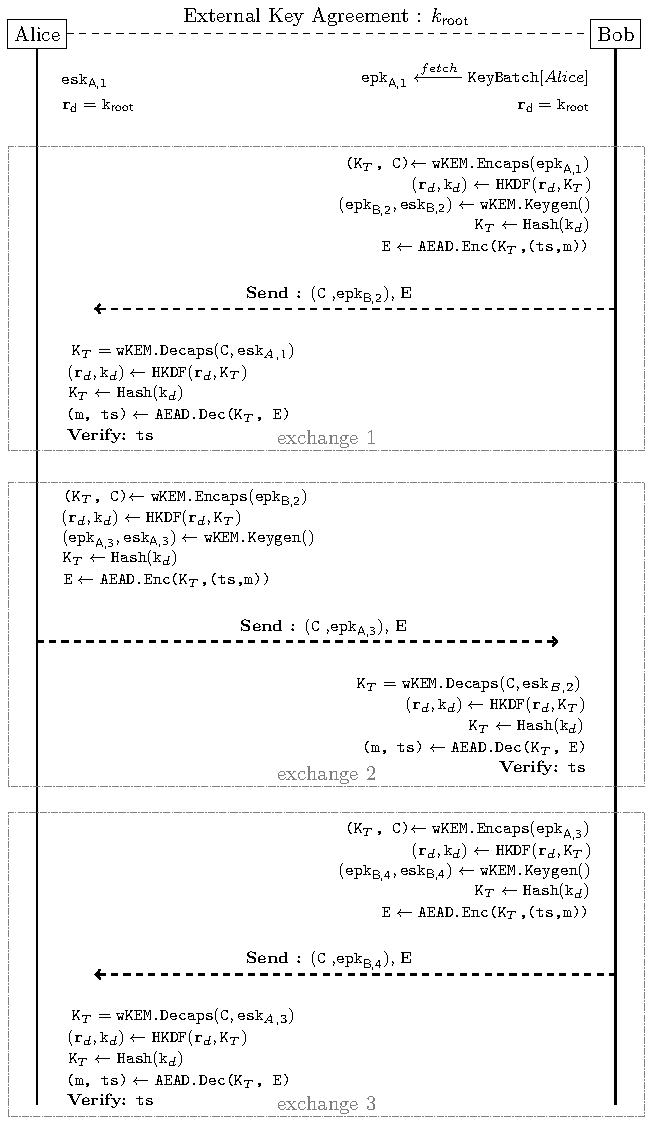
\includegraphics[height=\textheight]{kemdr.pdf}
    \caption{The KEM-double-ratchet protocol.}
    \label{DRProt}
\end{figure}

\begin{figure}[ht!]
\centering
% SI BESOINS DE PLACE:
\includegraphics[scale=0.85]{Graph_DR.pdf}
% SI PLACE OKAY:
%\includegraphics[]{article/Graph_DR.pdf}
    \caption{Graph of the Tamarin KEM-Double-Ratchet model.}
    \label{DRGraph}
\end{figure}

%\subsubsection{Tamarin model.} As shown in Fig.~\ref{DRGraph} we only perform three exchanges after the initialization of each participant. Normally Double-Ratchet offers an unbounded number of exchanges between users. However the reach of each security property that we model can be reduced to at most two exchanges (\textit{A property that has reach $r$ means that this property in exchange $k$ at most propagates to exchange $k \pm r$}). Thus we model KEM-Double Ratchet following Fig.~\ref{DRGraph}. We suppose that a secret has already been shared and thus each party initiates the cryptographic environment for the exchanges. To initialize the two users they use the rule \texttt{Init\_A} for the user having the role of A and \texttt{Init\_B} for the user having the role of B as shown in Fig.~\ref{DRGraph}. Then they derive secrets accordingly to Fig.~\ref{DRProt} to exchange their messages with rules depicted in Fig.~\ref{DRGraph}.
 %There is a slight difference between Fig.~\ref{DRProt} and KEM-Double Ratchet in  Tamarin. Since Tamarin has no built-in KEM we use asymmetric encryption to model it. Indeed the two approach are similar in case we suppose that the KEM is ideal. In order to replace the encapsulation we use an asymmetric encryption representing the challenge on a fresh variable that represents the shared secret built from a KEM.
\subsubsection{Tamarin model.} As shown in Figure~\ref{DRGraph} we only perform three exchanges of the KEM-double-ratchet protocol. Three exchanges are sufficient to verify all considered security properties as discussed in section~\ref{sec:verif}. Our KEM-DR model has nine transition rules:
\begin{compactitem}
\item \texttt{Init\_A} and \texttt{Init\_B}: each user get a secret preshared key and Bob gets an Alice's KEM ephemeral public key.
\item \texttt{Send\_B1}, \texttt{Send\_A}, and \texttt{Send\_B2}: the user encapsulates a fresh secret key with the current KEM public key, derives a new session key, encrypts the message, then sends it encrypted with the KEM ciphertext and a new ephemeral KEM public key.
\item \texttt{Recv\_A1}, \texttt{Recv\_B}, and \texttt{Recv\_A2}: the user receives a message, derives the new session key, and verifies the integrity.
\item \texttt{LeakState}: Reveals to the attacker the current user secrets.
\end{compactitem}
